%!TEX root = ../thesis.tex
%*******************************************************************************
%****************************** Fifth Chapter **********************************
%*******************************************************************************
\chapter{RealCodeが出題する演習問題の独自性評価}
\graphicspath{{Chapters_evaluation/Figs/}}
\label{section:ta_evaluation}


\ref{section:issue-classification}章にて述べたGitHubのイシューの抽出により,プログラミング演習問題に転用可能なイシューのデータセットを構築することができた.
しかし,教科書や授業で使用されている既存の演習問題とRealCodeが提供する演習問題がどう異なっているのかはまだ明らかになっていない.
そこで,大学でのプログラミングの講義においてティーチングアシスタント(TA)経験のある学生3名(PB1--PB3, 全て男性)によって,RealCodeが提供する演習問題の評価を行なった.
PB1とPB2は共に学部2年生を対象としたC言語の講義にて,TAとして授業中に様々な質問への回答や,テスト問題の作成を行なった経験がある.
PB3は学部3年生を対象とした別のC言語の講義において,C言語全般およびTCP/IPプロトコルについての質問対応と,最終レポートとプレゼンテーションの採点を担当していた.


\section{実験方法}
現在のRealCodeのプロトタイプに存在する116件のPythonの演習問題に対し,実験参加者はインターフェースにて提示される質問に対しに5段階で評価を行った(1: 全く同意しない -- 5: 強く同意する).
また,評価の理由を自由記述の形式で述べることのできる項目を質問の最後に設けた.
本実験に用いたインターフェースを図\ref{fig:originality-study-interface}に示す.

\begin{figure}[H]
 \centering
  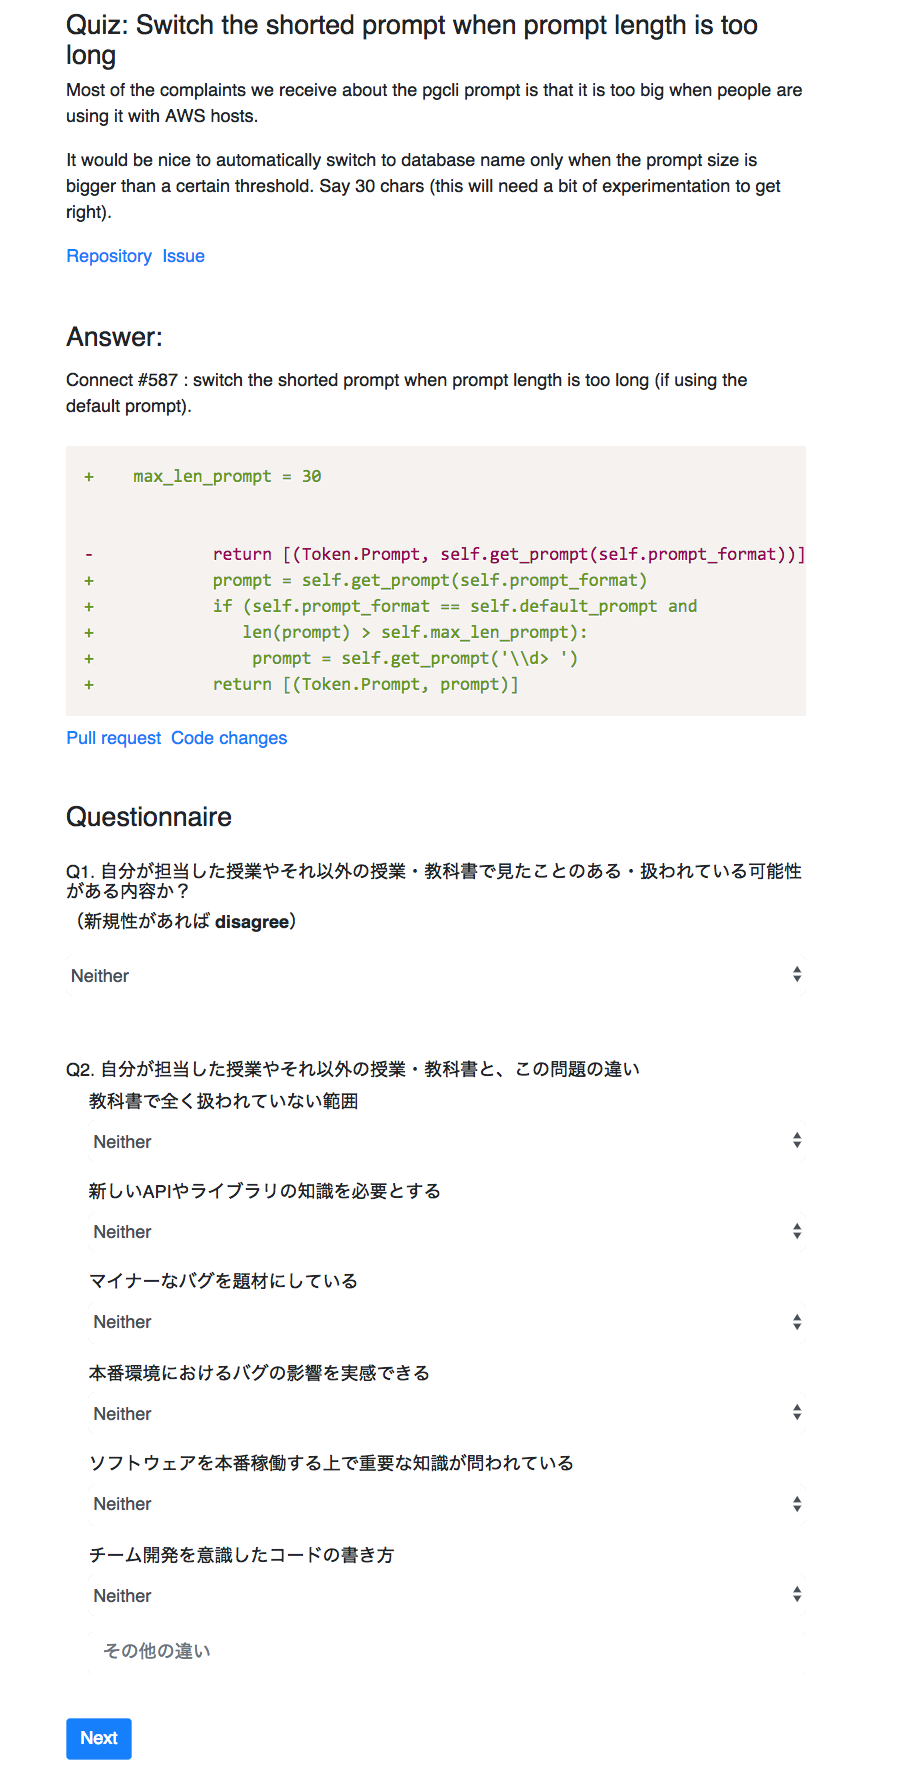
\includegraphics[width=0.8\columnwidth]{20190107-interface-originality-evaluation.png}
  \caption{評価に用いたインターフェース.}
  \label{fig:originality-study-interface}
\end{figure}

RealCodeが出題する演習問題の独自性評価にて行った質問を以下に示す.
\begin{itemize}
  \item[Q1.] 自分が担当した授業やそれ以外の授業・教科書で見たことのない・扱われている可能性がない内容か?
  \item[Q2.] 自分が担当した授業やそれ以外の授業・教科書と,この問題の違いは何か?
  \begin{itemize}
  	  \item Q2-1. 教科書で全く扱われていない範囲である
   	  \item Q2-2. 新しいAPIやライブラリの知識を必要とする
      \item Q2-3. あまり知られていないバグの修正を題材にしている
      \item Q2-4. 本番環境におけるバグの影響を実感できる
      \item Q2-5. ソフトウェアを本番稼働するための知識を必要とする
      \item Q2-6. チーム開発を意識したコードの書き方
  \end{itemize}
\end{itemize}

\section{実験結果}

\begin{table}[b]
  \centering
  \caption{TAによるシステム評価実験のQ2に関する,授業で扱われていないと判断された課題数.(表中の``agreed''は,「授業で扱われていないと判断された」を意味する. また,母数はQ1に対し3人中2人以上が「同意する」または「強く同意する」と回答し,かつ残りの一人が「全く同意しない」以外を回答した75問の演習問題である.)}
  \label{table:ta_evaluation_result}
  \begin{tabular}{l || c | c} \Xhline{3\arrayrulewidth}
      & \# of agreed & 率[\%] \\ \hline \hline
      Q2-1(教科書の範囲外) & 50 & 66.67 \\
      Q2-2(新しいAPIやライブラリ) & 40 & 53.33 \\
      Q2-3(知られていないバグの修正) & 35 & 46.67 \\
      Q2-4(バグの影響の実感) & 55 & 73.33 \\
      Q2-5(実際のシステムに必要な知識) & 49 & 65.33 \\
      Q2-6(チーム開発の実感) & 20 & 26.67 \\  
  \Xhline{3\arrayrulewidth}
  \end{tabular}
\end{table}

Q1に関して,3人中2人以上が「同意する」または「強く同意する」と回答し,かつ残りの一人が「全く同意しない」以外を回答した演習問題を,「授業・教科書では扱われていない課題」とみなすこととした.
これは半数以上の同意が得られたと同時に,強い反対がなかった演習問題を抽出するためである.
評価の結果,116問中75問(63.6\%)が授業・教科書では扱われていない課題と判断されたことがわかった.
その75問において,Q2の各選択肢に対してQ1と同様に,3人中2人以上が「同意する」または「強く同意する」と回答し,かつ残りの一人が「全く同意しない」以外を回答した演習問題の数を表\ref{table:ta_evaluation_result}に示す.
また,特に「授業・教科書では扱われていない課題」の割合が高いと評価された項目に関して考察を行う.

\subsection*{本番環境におけるバグの影響の体験}

本実験の結果,Q2-4(本番環境におけるバグの影響を実感できる)が最も同意を得られた項目であった.
RealCodeでは,実際のソフトウェアにおいて発生したバグを修正するイシューを転用した演習問題が多く提供されているからであると考えられる.
例えば,異なるOSで実行した際に発生するエラーを修正する演習問題において,RealCodeが実践的なバグ修正方法に関する知識を提供可能であることが示唆された.

\myquote{windowsとlinuxの違いを意識させられるし,OSの違いをうまく吸収するコーディングを学べる}{PB1}

また,実際のソフトウェア開発で頻発する問題の現実的な解決方法をRealCodeの演習問題が提供していることも確認された.

\myquote{不安定なコネクションという課題に対して実際に用いられている対策を学ぶことができる}{PB3}

\myquote{「この実行方法はサポートされていない」ということを明示的に出す経験は教科書や授業では扱わないと感じた}{PB1}


\subsection*{既存の学習環境で扱われていない内容の学習}

Q2-1(教科書で全く扱われていない範囲)はQ2-4に次いで同意が得られた項目であった.
例えばソフトウェアのテストを書くことは,既存の授業や教科書ではあまり扱われていない.
しかし,実際のソフトウェア開発においてテストは品質を保証する上で推奨される慣習である.
RealCodeではソフトウェアのテストに関する演習問題も提供されていることが確認された.

\myquote{授業でテストやテスティングライブラリを扱うことはあまりない}{PB2}

\myquote{テストを書くのは,既存のコードに合わせて書く必要があるので,その場で考える実践的な訓練になりそう}{PB1}

実際のソフトウェア開発では,ユーザにとって使いやすいシステムを実装することが求められる.
しかし,既存の教育素材においてシステムの利便性の向上を目指すといった正解のない演習問題はあまり見られない.
PB1の次のコメントは,RealCodeがシステムの使いやすさを向上するための知見を提供できることを示唆している.

\myquote{アルゴリズムの勉強というより,使いやすくするためにどうすればよいか?ということを考えさせられる部分が,授業や教科書では得られない体験}{PB1}




\subsection*{ソフトウェアの本番稼働に関する知識の習得}

また,Q2-5(ソフトウェアを本番稼働するための知識を必要とする)は,Q2-1に次いで同意が得られた項目であった.
ソフトウェアを安定的に本番稼働させるためには,コード変更を本番環境に反映させたり,本番環境のサーバの状況を監視したりする必要がある~\cite{carzaniga1998characterization}.
しかし,本番稼働に関する知見が教科書に記載されていることは少なく,RealCodeが既存の学習環境とは異なる視点から知見を提供できる可能性がある.

\myquote{continuous integrationができるように修正する経験は,授業や教科書ではあまりできない}{PB3}



























